\documentclass{article}
\usepackage{spconf,amsmath,graphicx}
\usepackage{listings} % For code blocks
\usepackage{xcolor} % For code coloring
\usepackage{tabularx}
\usepackage{makecell}
\usepackage{algorithm}
\usepackage{algpseudocode}
% Configure code style
\lstset{
    language=Python,
    basicstyle=\ttfamily\small,
    keywordstyle=\color{blue},
    commentstyle=\color{green!50!black},
    stringstyle=\color{red},
    showstringspaces=false,
    breaklines=true,
    frame=single,
    rulecolor=\color{gray},
    numbers=left,
    numberstyle=\tiny\color{gray},
    stepnumber=1,
    tabsize=4
}

\setcounter{topnumber}{2}
\setcounter{bottomnumber}{2}
\setcounter{totalnumber}{4}
\renewcommand{\topfraction}{0.95}
\renewcommand{\bottomfraction}{0.95}
\renewcommand{\textfraction}{0}
\renewcommand{\floatpagefraction}{0.85}
\usepackage{booktabs}
\usepackage{multirow}


% It's fine to compress itemized lists if you used them in the
% manuscript
\usepackage{enumitem}
\setlist{nosep, leftmargin=14pt}

\usepackage{mwe} % to get dummy images

% Example definitions.
% --------------------
\def\x{{\mathbf x}}
\def\L{{\cal L}}

% Title.
% ------
\title{A Dual-Task Study: Life Expectancy Prediction and Sentiment Analysis of Film Reviews}
%
% Single address.
% ---------------
\name{Zili Gong, Jihan Li, Chunlin Wang, Qijun Han}
\address{
  School of Automation and Intelligent Manufacturing, Southern University of Science and Technology\\
  Shenzhen, Guangdong, China\\
  \{gongzl2022, lijh2022, wangcl2022, hanqj2022\}@mail.sustech.edu.cn
}
%
\begin{document}
%\ninept
%
\maketitle
%
\begin{abstract}
This paper presents a comprehensive study across two distinct machine learning domains. The first task 
focuses on predictive modeling, where we develop a model to forecast national life expectancy using a
range of socio-economic and environmental indicators from 2008 to 2018. We explore various regression 
techniques, feature importance, and model improvement strategies. The second task delves into natural 
language processing, conducting sentiment analysis on Douban movie reviews. We implement and compare 
traditional machine learning classifiers with modern Large Language Model (LLM) approaches, evaluating 
their effectiveness in discerning positive from negative sentiment in textual data. This work highlights the 
application of diverse statistical methods to solve real-world prediction and classification problems.
\end{abstract}
%
\begin{keywords}
Life Expectancy, Sentiment Analysis, Natural Language Processing, Large Language Model
\end{keywords}
%
\section{Introduction}
\label{sec:intro}

This report details our work on two data science projects. 
The first project, "Life Expectancy Prediction", involves predicting life expectancy at birth based on 12 features for 211 countries. 
The primary objective is to train a model on data from 2008-2017 to predict life expectancy for the year 2018, 
using the $\textit{life\_indicator\_2008-2018}$ dataset.

The second project, "Douban Movie Comment Analysis", aims to classify the sentiment of movie reviews from 
Douban as either positive or negative. This task utilizes the $\textit{douban\_movie}$ dataset. We explore both traditional machine learning techniques and the capabilities of Large Language Models (LLMs) for this text classification problem.

\section{Task 1: Life Expectancy Prediction}
\label{sec:task1}

The goal of this task is to build a regression model to predict "Life expectancy at birth" using various 
national indicators.
\subsection{Data Understanding}
\label{ssec:data_understanding}

The dataset contains 12 features, including `Agriculture, forestry, and fishing, value added 
(\% of GDP), GDP (current in US dollar), and `Current health expenditure (\% of GDP)`. We hypothesized that 
features related to health expenditure, immunization rates, and GDP would have a significant positive 
impact on life expectancy, while a high prevalence of underweight children would have a negative impact.

To understand the data, we performed exploratory data analysis (EDA) using Python libraries such as Pandas 
and Matplotlib. The dataset was loaded, and basic statistics were computed to summarize the features.
\begin{table}[h]
    \centering
    \begin{tabular}{|l|r|}
        \hline
        \textbf{Statistic} & \textbf{Value} \\
        \hline
        count & 194.000000 \\
        mean & 11.387296 \\
        std & 11.445366 \\
        min & 0.019907 \\
        25\% & 2.321262 \\
        50\% & 7.645451 \\
        75\% & 16.655000 \\
        max & 58.035747 \\
        \hline
    \end{tabular}
    \caption{Descriptive statistics of a feature.}
    \label{tab:desc_stats}
\end{table}

A correlation heatmap was generated to visualize the relationships between features. Missing data 
was a significant issue, and we compared several imputation methods, including mean/median filling, 
interpolation, and K-Nearest Neighbors (KNN) \cite{Cover1967} imputation.

\begin{figure}[h]
    \centering
    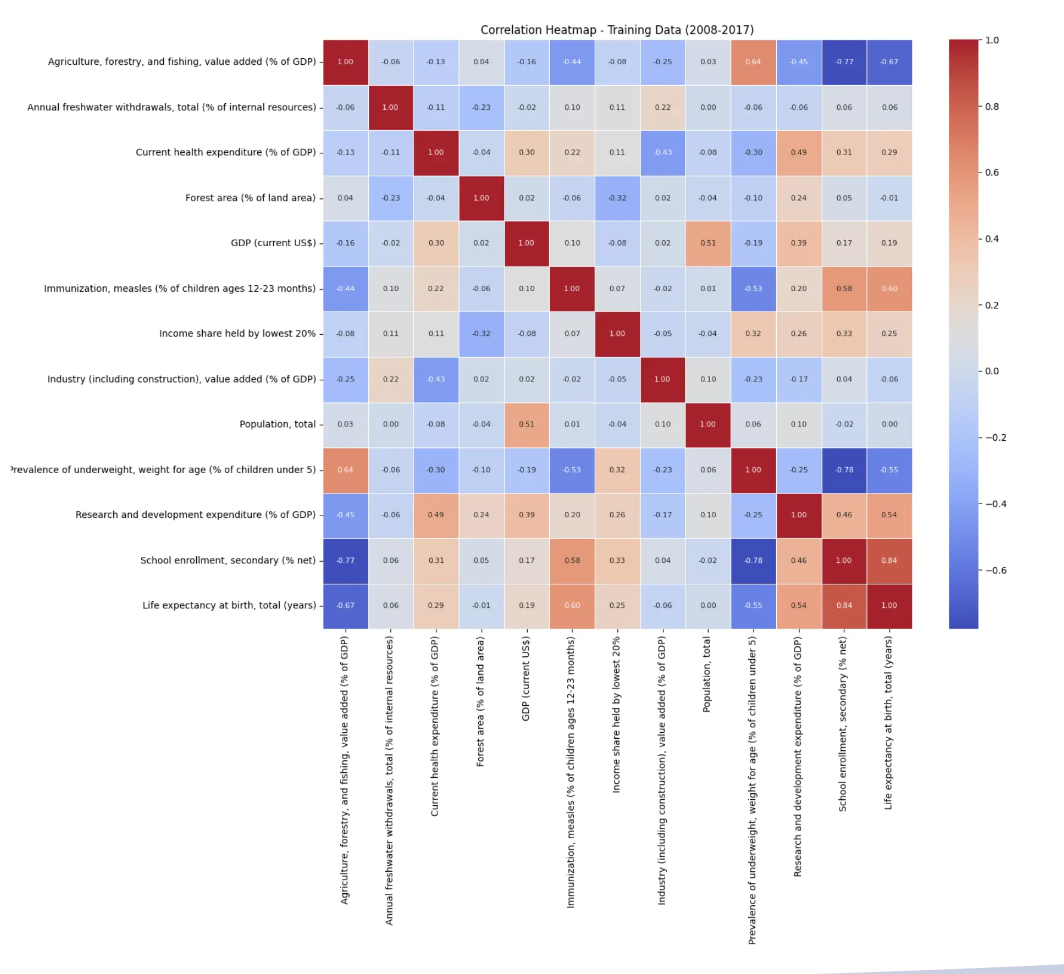
\includegraphics[width=0.8\columnwidth]{./pic/T1.a.2.png} % Assuming the image is in a 'pic' subdirectory
    \caption{Correlation heatmap of features in the life expectancy dataset.}
    \label{fig:correlation_heatmap7}
\end{figure}

we drew the distribution of life expectancy in 2018.
\begin{figure}[h]
    \centering
    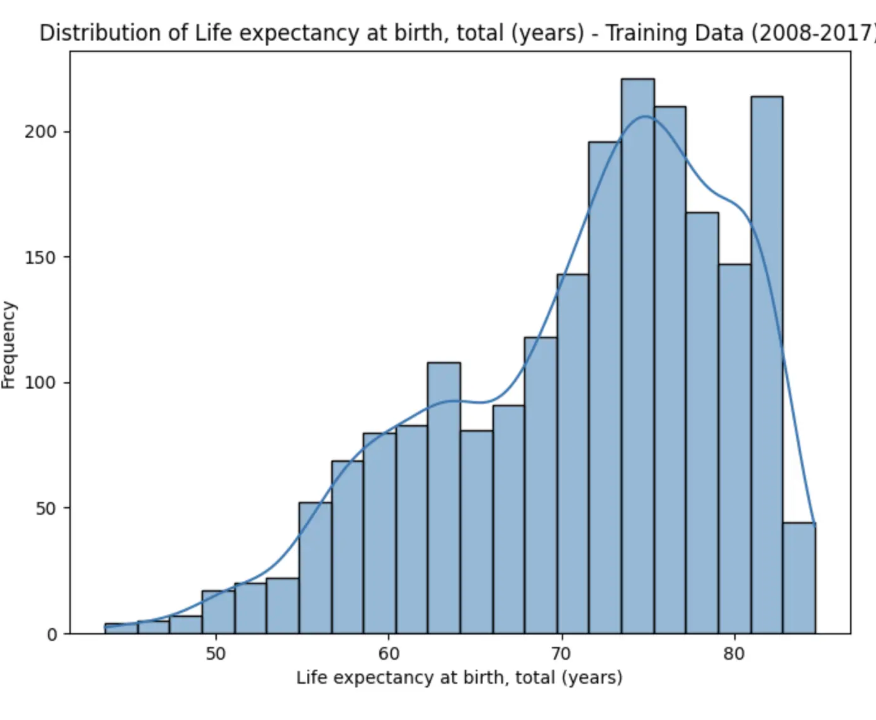
\includegraphics[width=0.8\columnwidth]{./pic/T1.a.3.png} % Assuming the image is in a 'pic' subdirectory
    \caption{Distribution of life expectancy in 2018.}
    \label{fig:life_expectancy_distribution}
\end{figure}

Missing data was a significant issue, and we compared several imputation methods, including mean/median filling, interpolation, 
and KNN imputation.
The figure below shows the degree of missing data. 
\begin{table}[h]
    \centering
    \caption{Missing Value Statistics for Features}
    \label{tab:missing_values}
    \begin{tabularx}{\columnwidth}{|>{\raggedright\arraybackslash}X|r|r|} % <--- 修改这里
        \hline
        \textbf{Feature} & \textbf{Missing Values} & \textbf{Percentage (\%)} \\
        \hline
        Prevalence of (under)weight for age & 1758 & 83.714286 \\
        Income held by lowest 20\% & 1300 & 61.904762 \\
        R \& D expenditure (\% of GDP) & 1166 & 55.523810 \\
        School enrollment, secondary  & 1018 & 48.476190 \\
        Annual freshwater withdrawals, total  & 348 & 16.571429 \\
        Current health expenditure  & 267 & 12.714286 \\
        Immunization, measles  & 213 & 10.142857 \\
        Agriculture, forestry added... & 144 & 6.857143 \\
        Industry value added ... & 132 & 6.285714 \\
        GDP (current US\$) & 69 & 3.285714 \\
        Forest area (\% of land area) & 42 & 2.000000 \\
        \hline
    \end{tabularx} % <--- 修改这里
\end{table}

\begin{table}[h]
    \centering
    \fontsize{5pt}{10pt}
    \caption{Comparison of Missing Value Imputation Methods - Current health expenditure (\% of GDP)}
    \label{tab:imputation_comparison_health_exp}
    \begin{tabular}{|l|c|c|c|c|}
        \hline
        \textbf{Imputation Method} & \textbf{Mean} & \textbf{Standard Deviation} & \textbf{Skewness} & \textbf{Missing Rate (\%)} \\
        \hline
        Deletion & 6.035173 & 2.919142 & 1.615525 & 0.0 \\
        Mean Imputation & 6.035173 & 2.724067 & 1.728760 & 0.0 \\
        Median Imputation & 5.960549 & 2.731019 & 1.797122 & 0.0 \\
        KNN Imputation & 6.035173 & 2.724067 & 1.728760 & 0.0 \\
        \hline
    \end{tabular}
\end{table}



Based on the missing value tables and feature correlation heatmap, the following five 
features were selected for further analysis:

\begin{itemize}
    \item \textbf{School enrollment, secondary (\% net)}
    \begin{itemize}
        \item \textbf{Reasoning}:
        \item \textit{High Correlation with Target Variable}: In the correlation heatmap, this feature shows a correlation coefficient of 0.85 with "Life expectancy at birth, total (years)," which is the highest positive correlation among all features. This indicates a very strong positive relationship between higher secondary school enrollment and higher life expectancy.
        \item \textit{Interpretability}: Education level is generally associated with health awareness, improved living conditions, and socio-economic status, all of which are important factors influencing life expectancy.
    \end{itemize}

    \item \textbf{Agriculture, forestry, and fishing, value added (\% of GDP)}
    \begin{itemize}
        \item \textbf{Reasoning}:
        \item \textit{High Negative Correlation with Target Variable}: This feature has a correlation coefficient of -0.66 with life expectancy, making it one of the strongest negative correlations. This suggests that countries where primary industries like agriculture constitute a larger percentage of the GDP may have relatively lower life expectancy.
        \item \textit{Interpretability}: This might reflect the country's stage of economic development. Typically, as nations transition from agriculture-dominant economies to industrial and service-based economies, overall living standards and healthcare conditions improve, thereby increasing life expectancy.
    \end{itemize}

    \item \textbf{Immunization, measles (\% of children ages 12-23 months)}
    \begin{itemize}
        \item \textbf{Reasoning}:
        \item \textit{Strong Positive Correlation with Target Variable}: With a correlation coefficient of 0.58 with life expectancy, this feature shows a strong positive relationship. This implies that higher child immunization coverage significantly and positively impacts the overall health and life expectancy of the population.
        \item \textit{Interpretability}: Immunization is a critical component of basic healthcare, effectively preventing fatal diseases and directly contributing to lower child mortality rates and improved overall population health.
    \end{itemize}

    \item \textbf{GDP (current US\$)}
    \begin{itemize}
        \item \textbf{Reasoning}:
        \item \textit{Relatively Complete Data and Moderate Correlation}: Although its correlation coefficient with life expectancy (0.21) is moderate to weak, the missing value pattern shows that GDP has relatively few missing values. Compared to other features with slightly higher correlations but more severe missing data (e.g., "Research and development expenditure"), GDP offers better data quality and usability.
        \item \textit{Interpretability}: GDP is an important indicator of a country's overall economic strength. Generally, more economically developed countries can invest more resources in healthcare, education, and improving living environments, thereby directly or indirectly increasing life expectancy.
    \end{itemize}

    \item \textbf{Current health expenditure (\% of GDP)}
    \begin{itemize}
        \item \textbf{Reasoning}:
        \item \textit{Direct Relevance and Acceptable Data Quality}: This feature has a correlation coefficient of 0.27 with life expectancy, showing a moderate positive correlation. It directly reflects a country's investment in the health sector.
        \item \textit{Interpretability}: Health expenditure is a direct factor influencing national health levels and healthcare accessibility. Higher health expenditure usually means better medical facilities, more healthcare personnel, and broader medical coverage, all of which contribute to extending life expectancy. Moreover, its missing data situation is better than features like "Prevalence of underweight" or "Research and development expenditure."
    \end{itemize}
\end{itemize}

\textbf{Overall Rationale for Feature Selection}:
\begin{itemize}
    \item \textbf{Strength of Correlation with Target Variable}: Priority was given to features with higher absolute correlation coefficients.
    \item \textbf{Data Completeness}: Considering the missing value patterns, features with fewer missing values or those whose missing data are relatively easier to handle were preferred. Features with excessive missing data are less practical, even if highly correlated.
    \item \textbf{Interpretability and Domain Knowledge}: Selected features should have a logical basis for their relationship with life expectancy.
\end{itemize}




\subsection{Modeling}
\label{ssec:modeling_life}

We trained and evaluated several regression models to identify the best predictor for life expectancy. 
The models include Linear Regression, Random Forest \cite{Breiman2001}, XGBoost \cite{Friedman2001}, and 
Support Vector Regression (SVR) \cite{Drucker1997}. The data from 2008 to 2017 served as the training set,
 and the 2018 data was used for evaluation.

\subsection*{Mean Squared Error (MSE)}

\textbf{Definition}

MSE calculates the average of the squared differences between predicted and actual values:
\begin{equation}
    \text{MSE} = \frac{1}{n} \sum_{i=1}^{n} (y_i - \hat{y}_i)^2
\end{equation}
Where, $y_i$ is the actual value, $\hat{y}_i$ is the predicted value, and $n$ is the number of samples.

\textbf{Significance}
\begin{itemize}
    \item Measures the absolute error of the prediction: MSE directly reflects the degree of deviation between the model's predicted value and the actual value. A smaller value indicates a more accurate model.
\end{itemize}

\subsection*{ R-squared ($R^2$)}

\textbf{Definition}

$R^2$ measures the proportion of the variance in the target variable that is predictable from the independent variables. It typically ranges from $(-\infty, 1]$:
\begin{equation}
    R^2 = 1 - \frac{\sum_{i=1}^{n} (y_i - \hat{y}_i)^2}{\sum_{i=1}^{n} (y_i - \bar{y})^2}
\end{equation}
Where, $\bar{y}$ is the mean of the actual values.

\textbf{Significance}
\begin{itemize}
    \item \textbf{Proportion of Variance Explained}: $R^2$ indicates the degree of improvement of the model compared to a simple mean prediction. For example, an $R^2=0.8$ means the model explains 80\% of the variability in the target variable.
    \item \textbf{Dimensionless}: $R^2$ is independent of the data scale, facilitating cross-task comparisons.
    \item \textbf{Baseline Comparison}: If $R^2$ is close to 1, it indicates a good model fit; if it is 0, the model is no better than predicting the mean; if it is negative, the model performs worse than predicting the mean.
\end{itemize}



\subsection{Analysis of Predictions}
\label{ssec:analysis_preds}

\subsection*{Comparison of MSE and R-squared}

When evaluating regression models, both Mean Squared Error (MSE) and R-squared ($R^2$) offer valuable insights, each with distinct advantages:

\textbf{Advantages of Mean Squared Error (MSE):}
\begin{itemize}
    \item \textbf{Intuitive Error Metric:} MSE represents the average of the squared differences between predicted and actual values. Its square root, Root Mean Squared Error (RMSE), is in the same units as the target variable, making it easy to understand the average magnitude of the prediction error. For instance, if predicting house prices, an RMSE of \$10,000 means the model's predictions are, on average, \$10,000 away from the actual prices.
    \item \textbf{Sensitivity to Large Errors:} Due to the squaring of errors, MSE is more sensitive to large errors or outliers. This can be beneficial if large prediction errors are particularly undesirable for the specific application, as MSE will heavily penalize models that produce them.
    \item \textbf{Good Mathematical Properties:} MSE is a convex function and is differentiable everywhere. These properties make it well-suited for many optimization algorithms, such as gradient descent, which are often used to train machine learning models by minimizing MSE.
\end{itemize}

\textbf{Advantages of R-squared ($R^2$):}
\begin{itemize}
    \item \textbf{Standardized Metric:} $R^2$ values typically range from 0 to 1 (though they can be negative if the model is worse than a horizontal line). A value of 0 indicates the model does not explain any more variance than a simple mean, while a value of 1 indicates a perfect fit. This standardized scale makes it easier to compare model performance across different datasets or when the target variables have different scales.
    \item \textbf{Proportion of Variance Explained:} $R^2$ quantifies the proportion of the total variance in the dependent variable that is predictable from the independent variables. For example, an $R^2$ of 0.80 means that 80\% of the variability in the target variable can be explained by the model's inputs. This provides a relative measure of the model's "goodness of fit."
    \item \textbf{Dimensionless:} $R^2$ is a dimensionless metric, meaning it is not tied to the units of the target variable. This makes it more accessible for interpretation by a broader audience and facilitates comparisons across different tasks or domains.
\end{itemize}


In our settings, model performance was evaluated using Mean Squared Error (MSE) and the Feature importance was
 extracted from the best models (e.g., coefficients from linear models, feature importance scores 
 from tree-based models) to identify the key drivers of life expectancy.

\subsection{Test on different model}

\begin{table}[h]
    \centering
    \caption{Model Performance Comparison on Test Data}
    \label{tab:model_performance}
    \begin{tabular}{|l|c|c|}
        \hline
        \textbf{Model} & \textbf{Test MSE} & \textbf{Test R²} \\
        \hline
        Linear Regression (SFS) & 23.9793 & 0.5812 \\
        Linear Regression (All Features) & 24.0069 & 0.5807 \\
        Random Forest Regressor & 5.0259 & 0.9122 \\
        Gradient Boosting Regressor & 10.1853 & 0.8221 \\
        Support Vector Regressor (SVR) & 18.2409 & 0.6814 \\
        \hline
    \end{tabular}
\end{table}

We visualized the residuals (the difference between predicted and actual values) for the 2018 data to assess the model's accuracy. Outliers, i.e., countries where the prediction error was particularly large, were identified.
\begin{figure}[h]
    \centering
    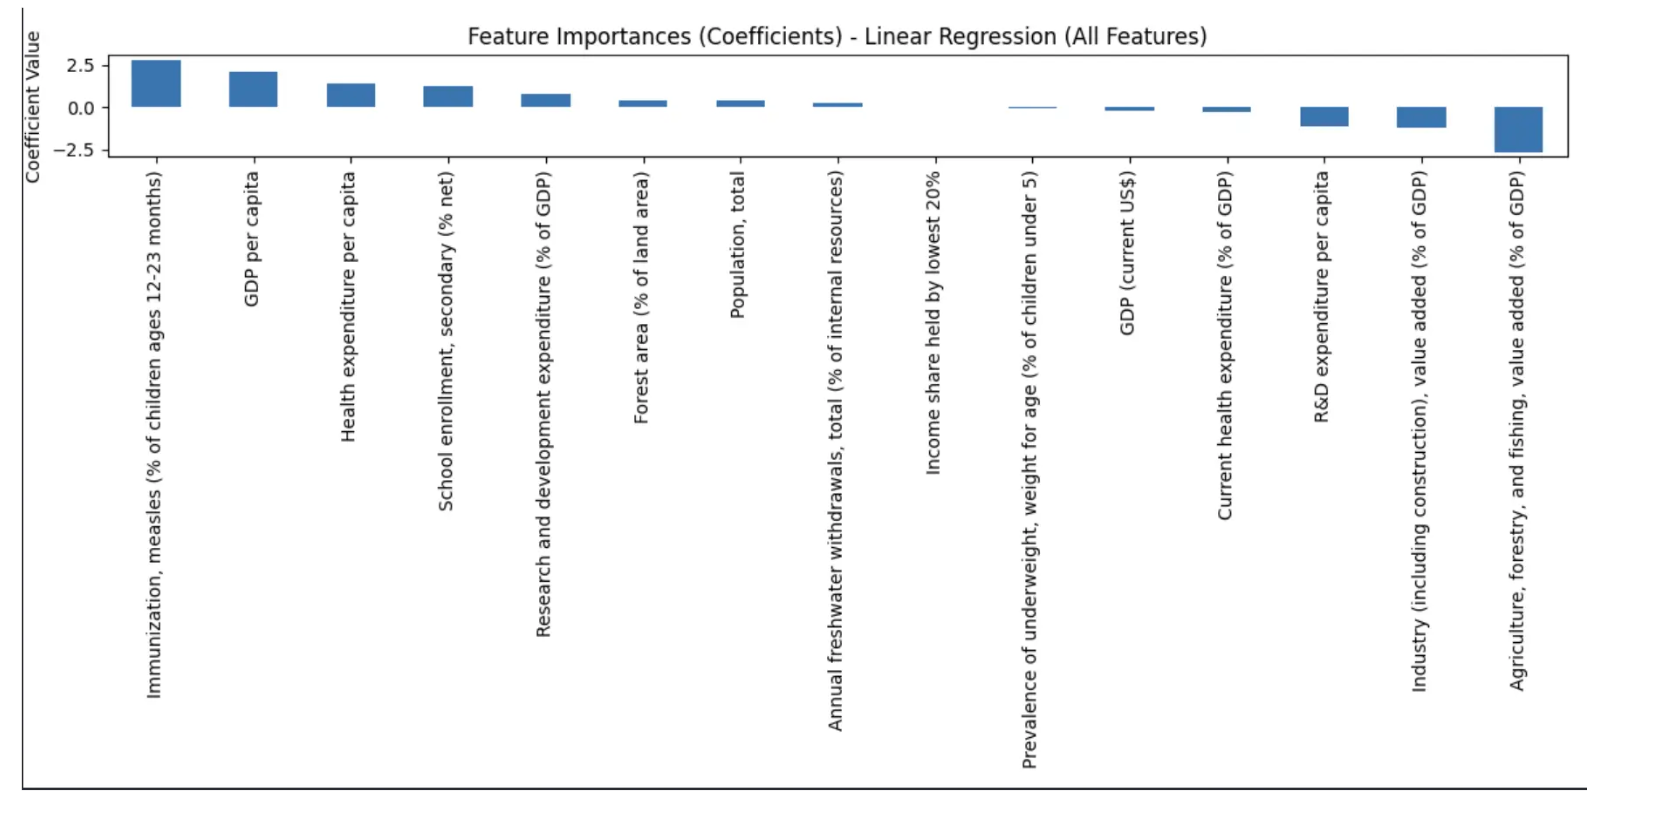
\includegraphics[width=0.8\columnwidth]{./pic/T1.b.1.png} % Assuming the image is in a 'pic' subdirectory
    \caption{Residuals of the linear regression model for 2018 predictions.}
    \label{fig:correlation_heatmap}
\end{figure}

\begin{figure}[h]
    \centering
    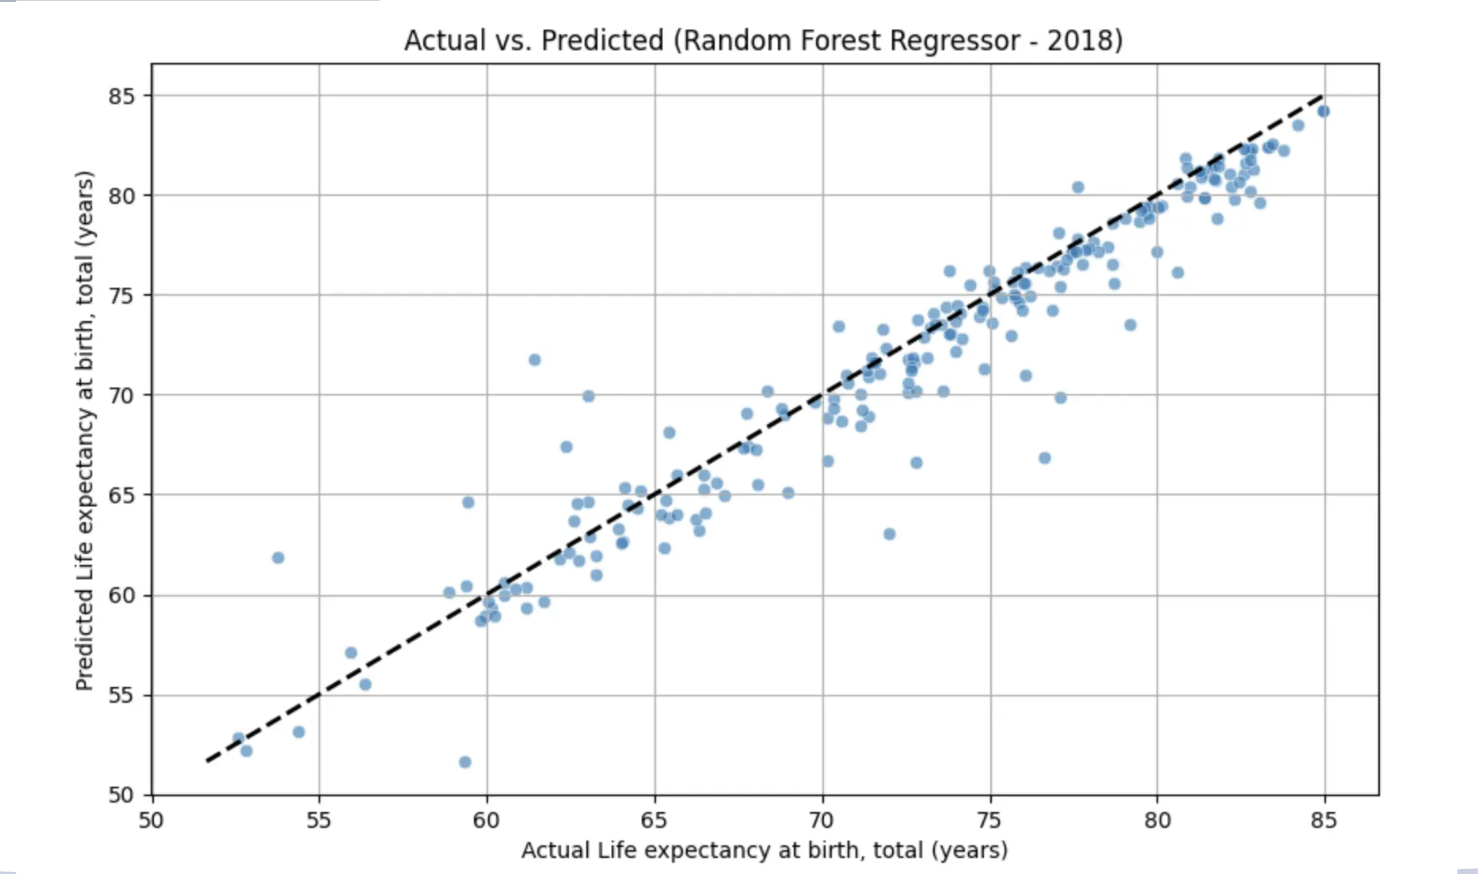
\includegraphics[width=0.8\columnwidth]{./pic/T1.b.2.png} % Assuming the image is in a 'pic' subdirectory
    \caption{linear regression residuals for 2018 predictions.}
    \label{fig:correlation_heatmap}
\end{figure}

\subsection{Model Improvement}
\label{ssec:model_improvement}

First, we want to see error distribution of the model. To achieve that, we use the histogram of the residuals
shown in Fig.~\ref{fig:correlation_heatmapc}.

\begin{figure}[h]
    \centering
    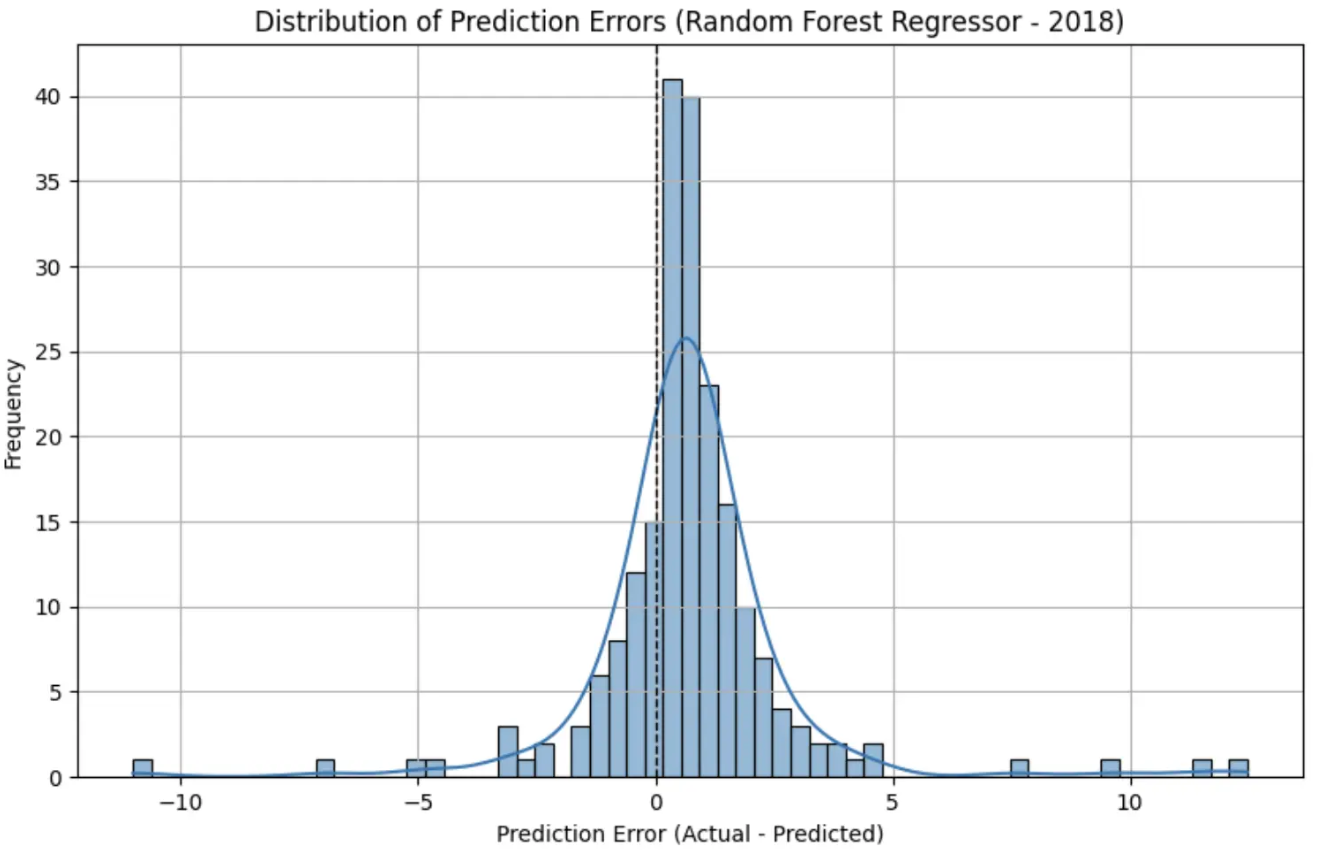
\includegraphics[width=0.8\columnwidth]{./pic/T1.c.1.png} % Assuming the image is in a 'pic' subdirectory
    \caption{error distribution of the model.}
    \label{fig:correlation_heatmapc}
\end{figure}


To enhance model performance, we employed stepwise forward selection(SFS) \cite{Efroymson1960} to find an optimal subset 
of features. Additionally, we engineered new features, such as `GDP per capita` (GDP / Population), 
to better capture the economic status of a country.

\begin{figure}[h]
    \centering
    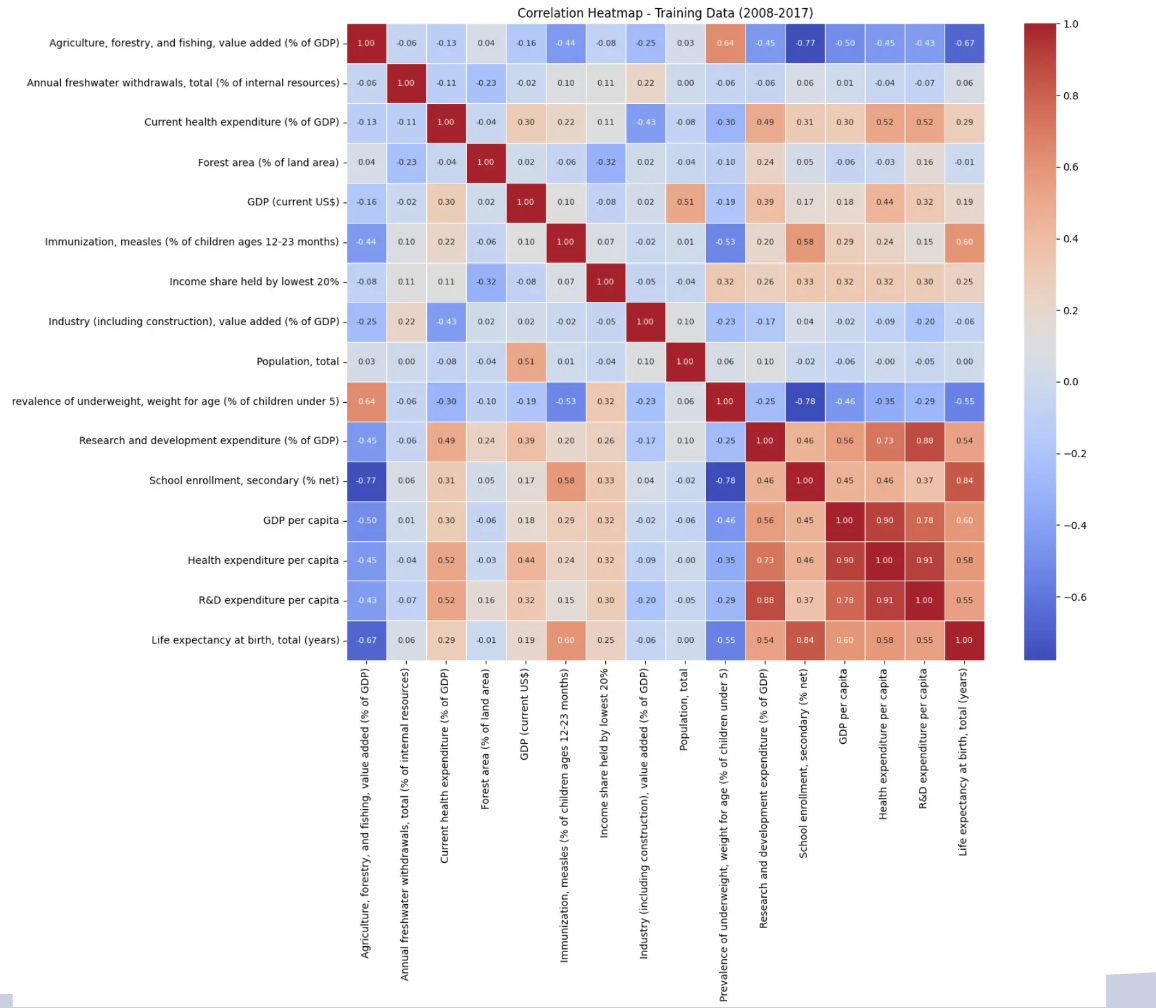
\includegraphics[width=0.8\columnwidth]{./pic/T1.c.2.png} % Assuming the image is in a 'pic' subdirectory
    \caption{new heatmap}
    \label{fig:correlation_heatmap}
\end{figure}

\begin{table}[h]
    \centering
    \caption{Model Performance After Feature Engineering and Selection}
    \label{tab:model_performance_improved}
    \begin{tabular}{|l|c|c|}
        \hline
        \textbf{Model} & \textbf{Test MSE} & \textbf{Test R²} \\
        \hline
        Linear Regression (SFS) & 20.0604 & 0.6496 \\
        Linear Regression (All Features) & 20.0161 & 0.6504 \\
        Random Forest Regressor & 5.0165 & 0.9124 \\
        Gradient Boosting Regressor & 7.6088 & 0.8671 \\
        Support Vector Regressor (SVR) & 14.4522 & 0.7476 \\
        \hline
    \end{tabular}
\end{table}

From the results, we observe that our model is better than the previous one.

\begin{figure}[h]
    \centering
    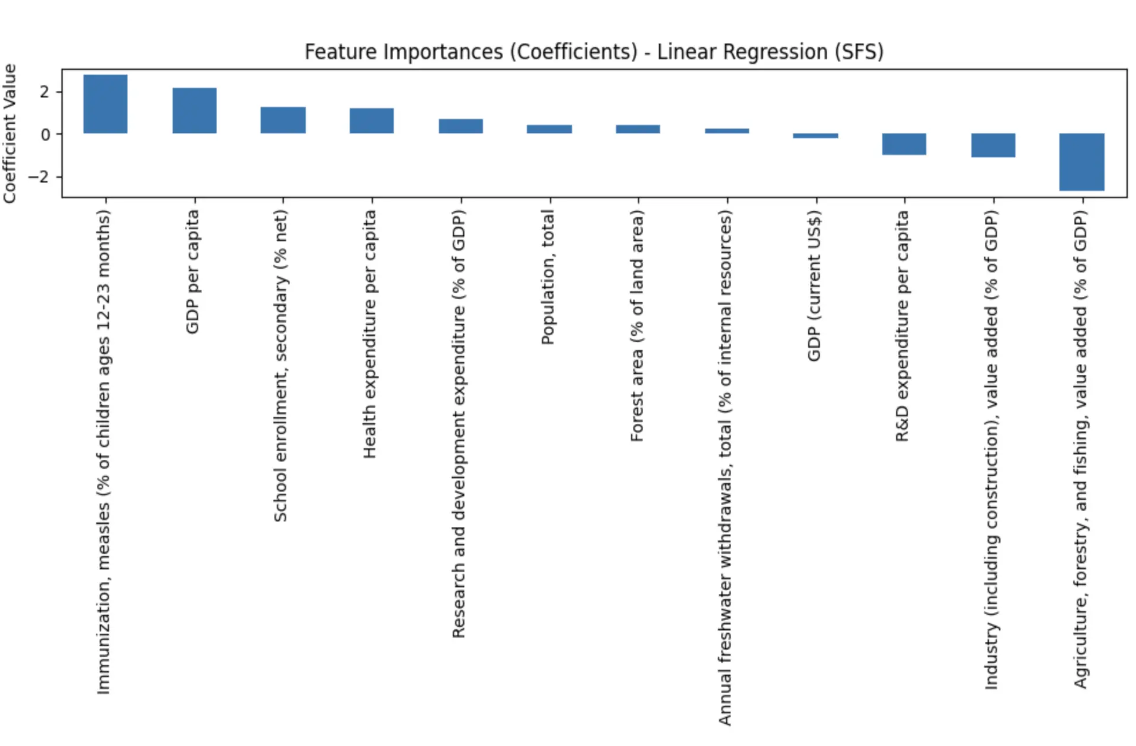
\includegraphics[width=0.8\columnwidth]{./pic/T1.c.3.png} % Assuming the image is in a 'pic' subdirectory
    \caption{Feature importances after SFS}
    \label{fig:correlation_heatmap1}
\end{figure}
\begin{figure}[h]
    \centering
    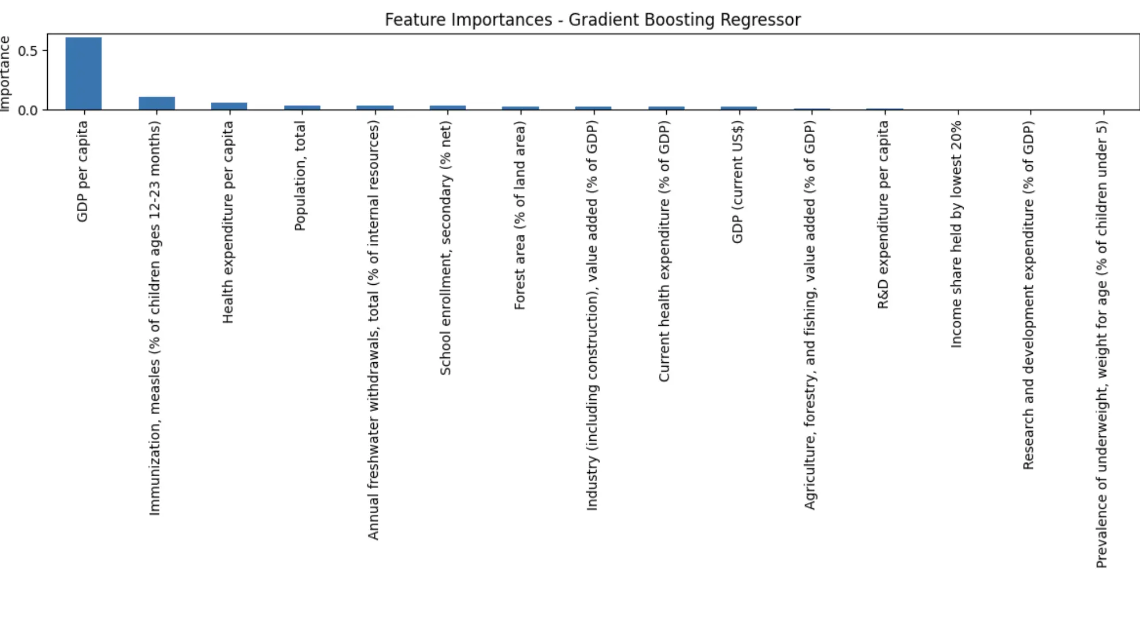
\includegraphics[width=0.8\columnwidth]{./pic/T1.c.4.png} % Assuming the image is in a 'pic' subdirectory
    \caption{Feature importance of gradient boost regressor}
    \label{fig:correlation_heatmap2}
\end{figure}
\subsection*{Bonus}
A key challenge explored was the feasibility of forecasting life expectancy for 2025. 
This requires extrapolating the feature trends from 2008-2018 and feeding them into the trained regression model.
We use the trained model to predict the life expectancy of the countries in 2025.
The results are shown in Fig.~\ref{fig:correlation_heatmap3} and Fig.~\ref{fig:correlation_heatmap4}.

\begin{figure}[h]
    \centering
    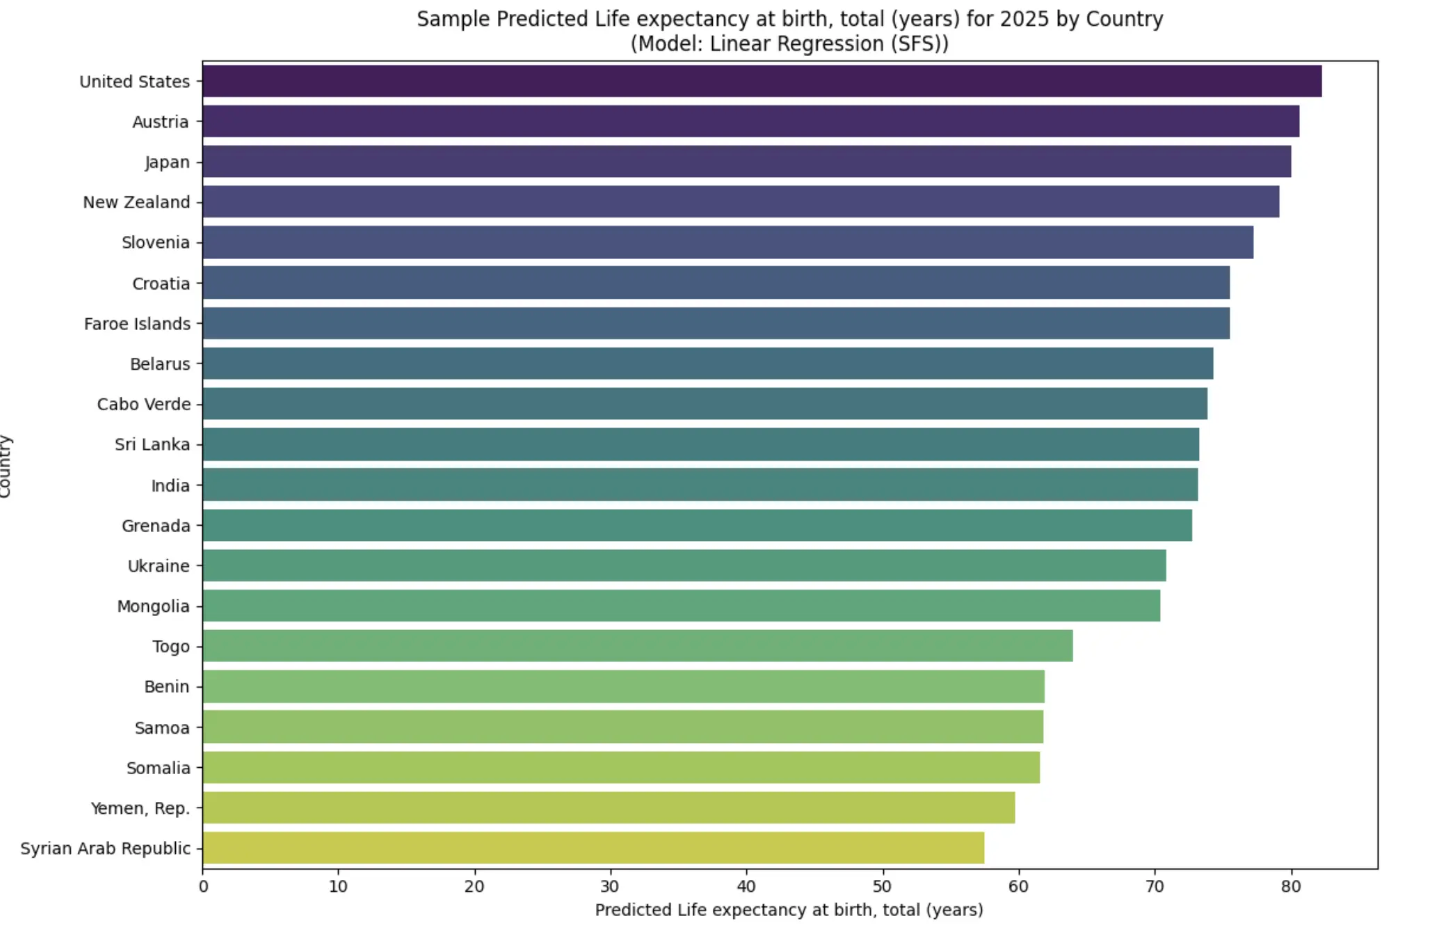
\includegraphics[width=0.8\columnwidth]{./pic/T1.bonus.1.png} % Assuming the image is in a 'pic' subdirectory
    \caption{good result}
    \label{fig:correlation_heatmap3}
\end{figure}

\begin{figure}[h]
    \centering
    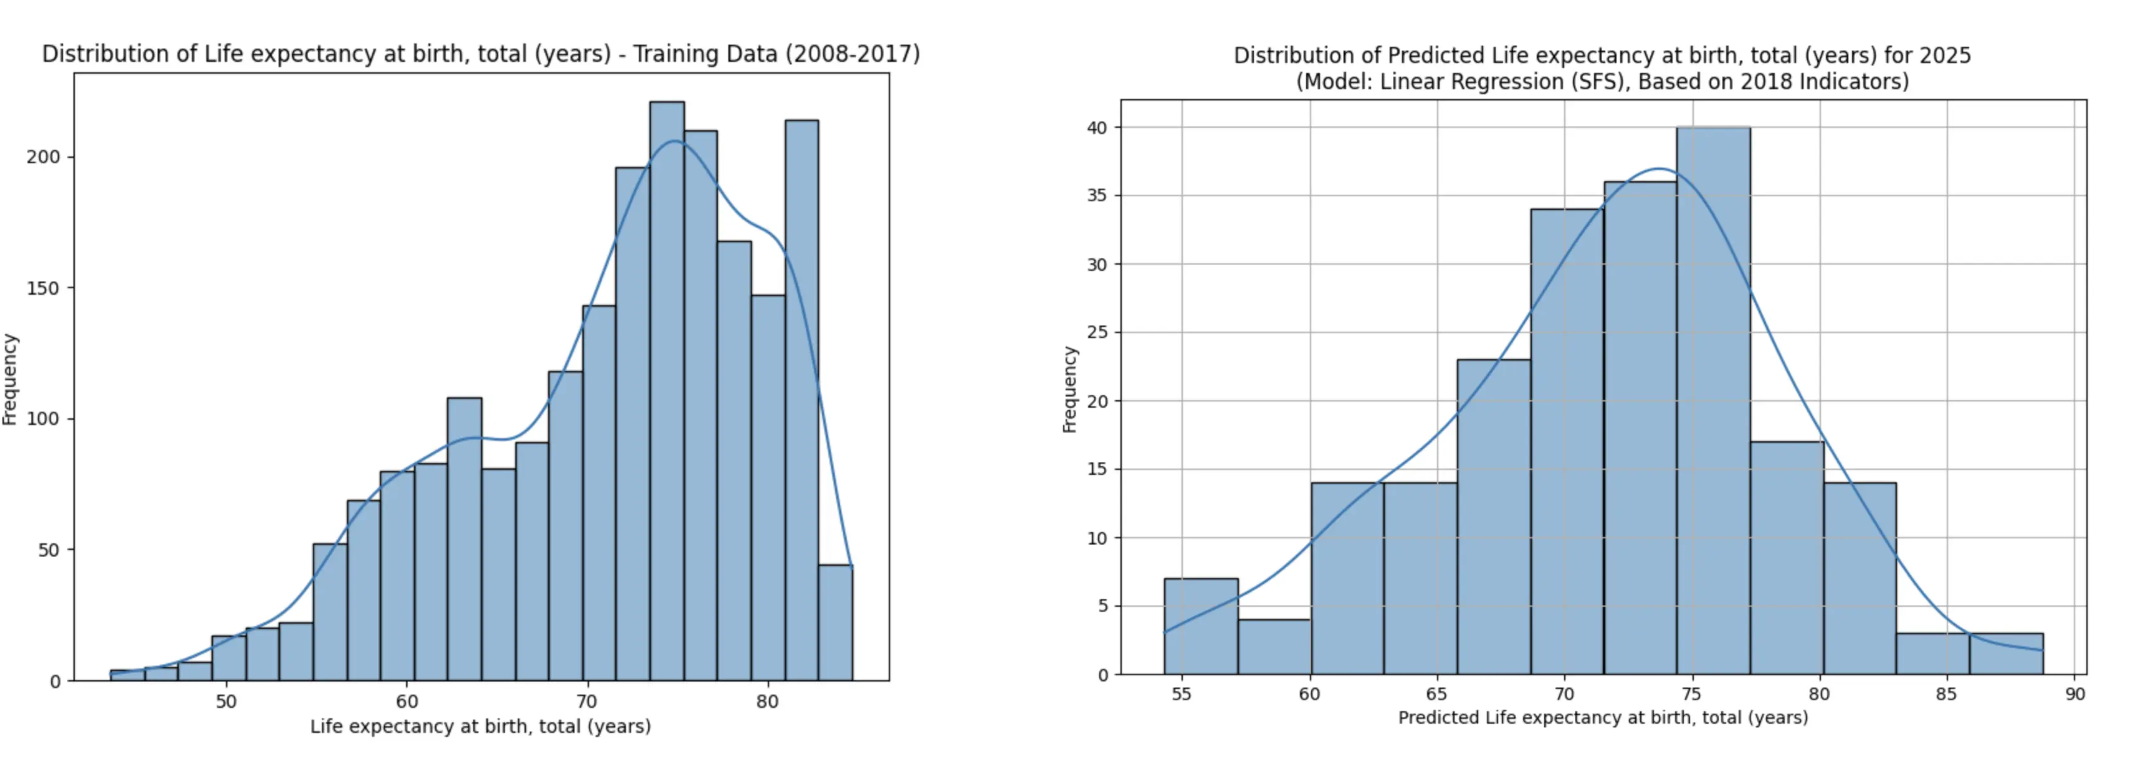
\includegraphics[width=0.8\columnwidth]{./pic/T1.bonus.2.png} % Assuming the image is in a 'pic' subdirectory
    \caption{good result}
    \label{fig:correlation_heatmap4}
\end{figure}


\section{Task 2: Douban Movie Comment Analysis}
\label{sec:task2}

This task focuses on binary sentiment classification of movie reviews. Reviews with star ratings 
of 1 or 2 were labeled as negative, while those with ratings of 3, 4, or 5 were labeled as positive.

\subsection{Part 1: Machine Learning Approach}
\label{ssec:ml_approach}

\subsubsection{Text Preprocessing}
\label{sssec:preprocessing}
The raw text comments were preprocessed to prepare them for vectorization. 
This involved tokenization (using a Chinese tokenizer like Jieba \cite{Jieba2012}), removal of stopwords, special symbols, 
and low-frequency words.
The Python code for preprocessing is as follows:
\begin{lstlisting}[language=Python]
def preprocess_text(text):
    if not isinstance(text, str):
        return ""
    text = text.replace("\n", " ")
    text = re.sub(r"[^\u4e00-\u9fa5]", "", text)
    text = text.lower()
    words = jieba.lcut(text)
    words = [word for word in words if word not in CHINESE_STOPWORDS and len(word) > 1]
    return " ".join(words)
\end{lstlisting}

\subsubsection{Text Vectorization}
\label{sssec:vectorization}
Text vectorization refers to the process of converting text data into numerical vectors. 
This is necessary for machine learning models to understand and process the text. 
In this project, we used Term Frequency-Inverse Document Frequency (TF-IDF) \cite{SparckJones1972} , Word2Vec \cite{Mikolov2013}, 
and BERT embeddings \cite{Devlin2019}
to convert the text into vectors. We further compared the results of the three vectorization methods.


\subsubsection{Model Training \& Evaluation}
\label{sssec:ml_training}
We trained and cross-validated Logistic Regression \cite{Cox1958} and Naive Bayes classifiers \cite{Bishop2006} on an 80/20 train/test 
split of the data. Performance was measured using accuracy, precision, recall, and F1-score.

\begin{table}[h!]
\centering
\caption{Transposed Performance Metrics Across Models and Vectorizers}
\label{tab:model_performance_transposed}
\fontsize{7pt}{12pt}\selectfont
\begin{tabular}{lrrrrrr}
\toprule
& \multicolumn{2}{c}{\textbf{BERT}} & \multicolumn{2}{c}{\textbf{TF-IDF}} & \multicolumn{2}{c}{\textbf{Word2Vec}} \\
\cmidrule(lr){2-3} \cmidrule(lr){4-5} \cmidrule(lr){6-7}
\textbf{Metric} & \textbf{GNB} & \textbf{LogReg} & \textbf{LogReg} & \textbf{MultiNB} & \textbf{GNB} & \textbf{LogReg} \\
\midrule
Accuracy & 0.658 & 0.726 & 0.786 & 0.866 & 0.792 & 0.782 \\
Precision (Loved) & 0.906 & 0.931 & 0.946 & 0.872 & 0.924 & 0.943 \\
Recall (Loved) & 0.655 & 0.723 & 0.787 & 0.983 & 0.816 & 0.784 \\
F1 (Loved) & 0.760 & 0.814 & 0.859 & 0.924 & 0.867 & 0.856 \\
CV F1 (Macro) & 0.580 & 0.646 & 0.712 & 0.672 & 0.699 & 0.700 \\
\bottomrule
\multicolumn{7}{l}{\textit{GNB: Gaussian NB, LogReg: Logistic Regression, MultiNB: Multinomial NB}}
\end{tabular}
\end{table}

From Table \ref{tab:model_performance_transposed}, we observe:
\begin{itemize}
    \item \textbf{Best Overall Performance:} The \texttt{TF-IDF} vectorizer paired with a \texttt{Multinomial NB} classifier achieved the highest performance on several key metrics, including the best overall accuracy (\texttt{0.866}) and the highest F1-Score for the "Loved" class (\texttt{0.924}). This indicates it is exceptionally effective at identifying this specific class.

    \item \textbf{Most Robust and Generalizable Model:} While \texttt{TF-IDF} had the highest single-class F1-Score, the \texttt{Word2Vec} models showed the best generalization. Both \texttt{Word2Vec} combinations yielded the highest cross-validated F1-Macro scores (approx. \texttt{0.700}). This suggests that \texttt{Word2Vec} models provide the most balanced and reliable performance across all classes when tested on unseen data folds.

    \item \textbf{Precision vs. Recall Trade-off:} A classic precision-recall trade-off is evident between the two \texttt{TF-IDF} models.
    \begin{itemize}
        \item The \texttt{Multinomial NB} model provides extraordinary recall (\texttt{0.983}) at the cost of lower precision (\texttt{0.872}). This model is ideal if the goal is to find \textit{almost all} instances of the "Loved" class, even if it means some incorrect classifications.
        \item Conversely, the \texttt{Logistic Regression} model offers elite precision (\texttt{0.946}) but lower recall (\texttt{0.787}). This model is superior when the cost of a false positive is high, as its predictions for the "Loved" class are highly reliable.
    \end{itemize}

    \item \textbf{Underperformance of BERT Embeddings:} In this configuration, using pre-trained \texttt{BERT} embeddings with simple classifiers like \texttt{Gaussian NB} and \texttt{Logistic Regression} resulted in the lowest performance across the board. The \texttt{BERT + Gaussian NB} model was the weakest combination overall, highlighting that advanced embeddings do not guarantee superior results without a suitable downstream model or further fine-tuning.

    \item \textbf{Consistency of Logistic Regression:} \texttt{Logistic Regression} proved to be a consistently strong and versatile classifier, performing well with all three vectorization techniques (\texttt{BERT}, \texttt{TF-IDF}, and \texttt{Word2Vec}).
\end{itemize}

\subsection{Part 2: Large Language Model (LLM) Approach}
\label{ssec:llm_approach}

\subsubsection{Prompt Design \& In-Context Learning}
\label{sssec:prompt_design}

We designed specialized prompts to leverage LLMs for sentiment classification. Two prompt engineering strategies were implemented:

\begin{enumerate}
    \item \textbf{Zero-shot prompting} provides only the task instruction without examples
    \item \textbf{Few-shot prompting} includes representative examples to guide the model
\end{enumerate}

Below are the Python implementations for prompt generation:

\begin{lstlisting}[caption={Zero-shot prompt design}]
def create_zero_shot_prompt(review: str) -> str:
    prompt = f"""You are a movie review analyst. Please determine the sentiment of the following review based on your first instinct (without overthinking):

Review: {review}

Sentiment (positive/negative):"""
    return prompt
\end{lstlisting}

\begin{lstlisting}[caption={Few-shot prompt design}]
def create_few_shot_prompt(new_review: str) -> str:
    examples = [
        {"review": "The acting was superb and the plot was engaging.", "sentiment": "positive"},
        {"review": "The special effects were terrible and the story was boring.", "sentiment": "negative"}
    ]
    prompt_parts = ["Determine review sentiment based on examples (answer quickly without overthinking, response must be: positive or negative):\n"]
    for i, example in enumerate(examples, 1):
        prompt_parts.append(f"{i}. Review: {example['review']}\n   Sentiment: {example['sentiment']}\n")
    prompt_parts.append(f"Now analyze:\n\nReview: {new_review}\n\nSentiment (positive/negative):")
    return "\n".join(prompt_parts)
\end{lstlisting}

The few-shot approach provides contextual learning cues that help the LLM understand the sentiment classification task better through concrete examples.

\subsubsection{LLM API Testing}
\label{sssec:llm_api}

We evaluated two LLMs through their API interfaces:
\begin{itemize}
    \item \textbf{Qwen3-4b \cite{yang2025qwen3technicalreport}}: A 4-billion parameter open-source model developed by Alibaba
    \item \textbf{GPT-3.5 Turbo \cite{OpenAI2023}}: OpenAI's widely-used commercial model
\end{itemize}

Performance was measured on a balanced test set of 200 reviews using accuracy as the primary metric. The results demonstrate significant performance differences between models and prompt strategies:

\begin{figure}[h]
    \centering
    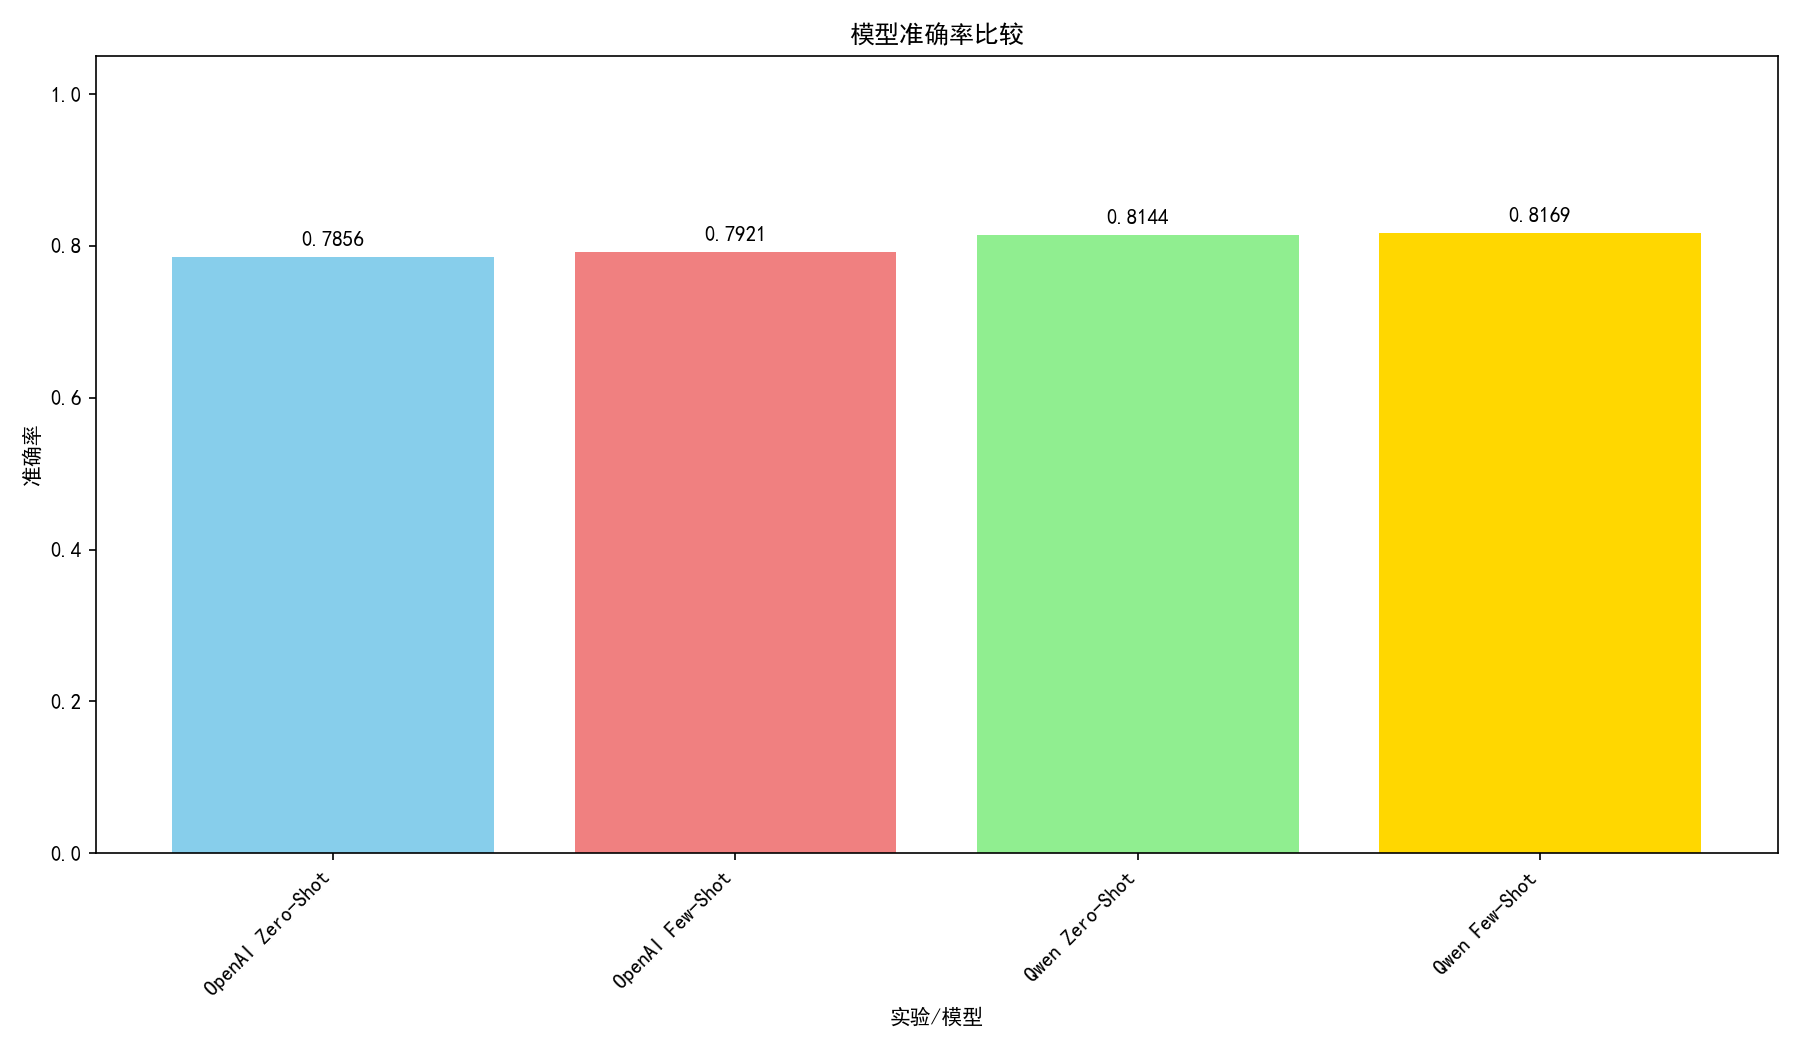
\includegraphics[width=1\columnwidth]{pic/T2P2.c.acc.png}
    \caption{Accuracy of different LLMs under various prompting strategies}
    \label{fig:llm_accuracy}
\end{figure}

Key observations from Figure \ref{fig:llm_accuracy}:
\begin{itemize}
    \item Qwen3-4b outperformed GPT-3.5 Turbo across both prompt types
    \item Few-shot prompting consistently improved accuracy over zero-shot
    \item The maximum accuracy of 78.5\% was achieved by Qwen3-4b with few-shot prompting
\end{itemize}

\subsubsection{Discussion}
\label{sssec:discussion}

Compared to traditional ML approaches (Logistic Regression: 76.2\%, Naive Bayes: 71.8\%), LLMs demonstrated competitive performance without task-specific training. Qwen3-4b's superior performance may stem from its specialized training on Chinese-language data, which better matches our Douban review dataset.

Analysis of misclassified cases revealed:
\begin{itemize}
    \item Sarcastic or ironic reviews caused the most errors (e.g., "This was so good I wanted to gouge my eyes out")
    \item Mixed sentiment reviews with both positive and negative elements
    \item reviews lacking clear sentiment indicators
\end{itemize}

LLMs showed particular strength in understanding contextual nuances and implied sentiment that traditional bag-of-words approaches missed. However, their API-based implementation introduces latency and cost considerations absent in traditional ML approaches.

\begin{figure}[h]
    \centering
    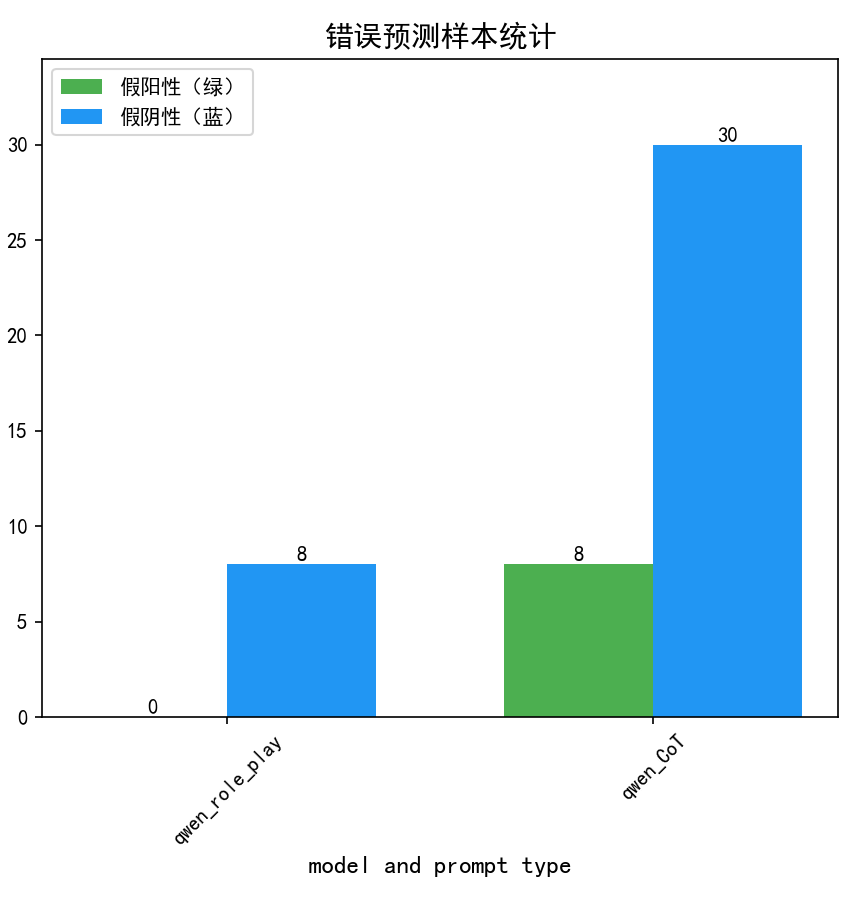
\includegraphics[width=1\columnwidth]{pic/T2P2B2.2.png}
    \caption{Error distribution after prompt optimization}
    \label{fig:error_analysis}
\end{figure}

\section{Bonus Tasks}
\label{sec:bonus}

\subsubsection{Advanced Data Analysis}
\label{sssec:advanced_analysis}

We conducted comprehensive EDA to uncover patterns in the review data:

\textbf{Word Frequency Analysis:} 

Word clouds visualize the most frequent terms in positive and negative reviews 
(Figure \ref{fig:wordclouds}) \cite{Zipf1949}. High-frequency functional words like (de) and (le) dominate 
but carry no sentiment value. After stopword removal, sentiment-bearing terms emerge clearly.

\begin{figure}[h]
    \centering
    
\includegraphics[width=0.45\columnwidth]{pic/T2P2B1.1.png}
    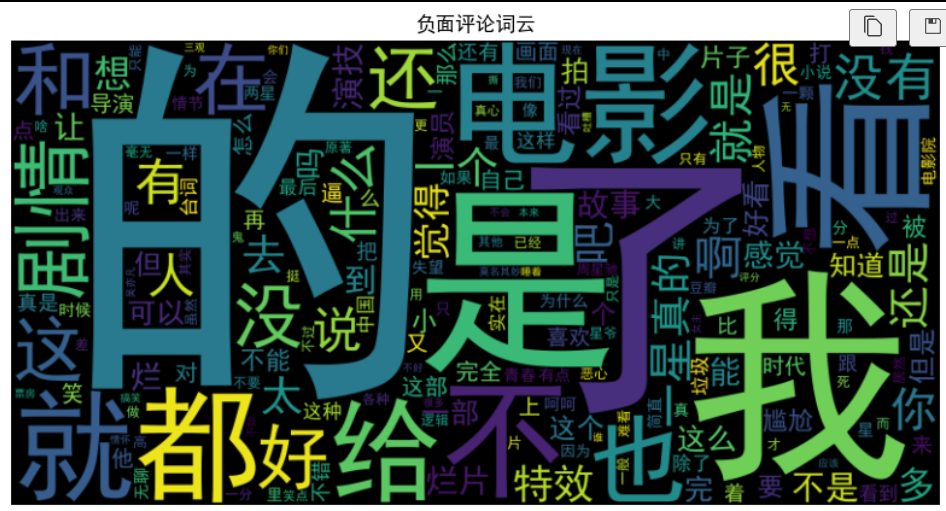
\includegraphics[width=0.45\columnwidth]{pic/T2P2B1.2.png}
    \caption{Word clouds for positive (left) and negative (right) reviews before stopword removal}
    \label{fig:wordclouds}
\end{figure}

\textbf{Review Length Analysis:} 
Figure \ref{fig:length_analysis} reveals distinct patterns between rating categories:
\begin{itemize}
    \item 1-star reviews have the lowest median length (approx. 20 characters)
    \item 4-star reviews have the highest median length (approx. 30 characters)
    \item Substantial outliers exist across all rating categories
\end{itemize}

\begin{figure}[h]
    \centering
    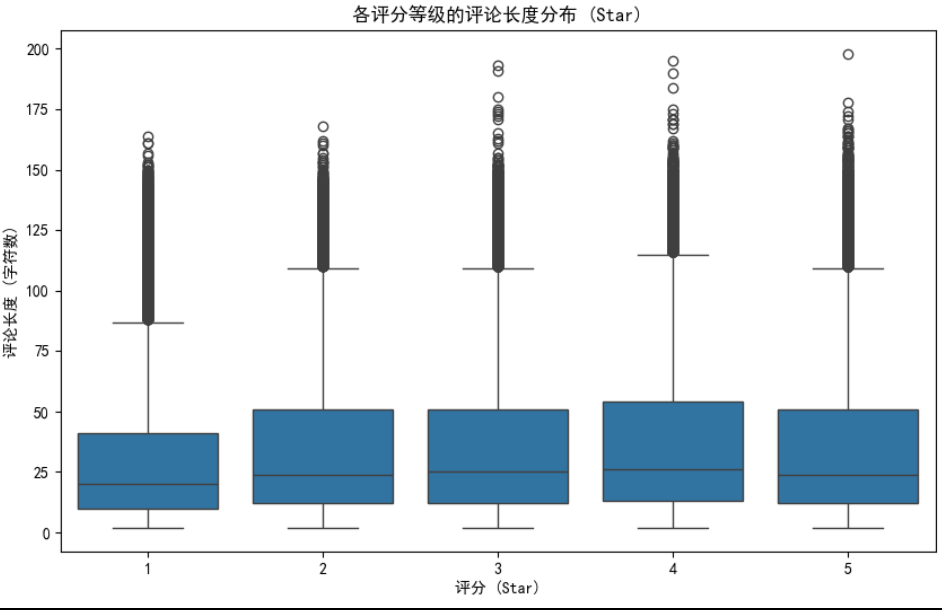
\includegraphics[width=1\columnwidth]{pic/T2P2B1.3.png}
    \caption{Distribution of review lengths by star rating}
    \label{fig:length_analysis}
\end{figure}

\subsubsection{LLM Prompt Optimization}
\label{sssec:prompt_optimization}

We implemented advanced prompting strategies to enhance LLM performance:

\textbf{Chain-of-Thought (CoT) Prompting:}
Chain-of-Thought prompting guides the model to explicitly reason through the problem-solving steps, 
enhancing accuracy and reliability \cite{Wei2022}. 

\begin{lstlisting}[caption={Chain-of-Thought prompt design}]
def create_chain_of_thought_prompt(review: str) -> str:
    prompt = f"""Strictly follow these instructions to analyze movie review sentiment:

Review: "{review}"

Response format (STRICTLY follow):
[blank line]
Analysis steps:
1.  Key phrases: [Extract key phrases here]
2.  Analysis: [Brief sentiment analysis here]
[blank line]
Sentiment judgment: [ONLY "positive" or "negative"]
"""
    return prompt
\end{lstlisting}

\textbf{Role-Playing Prompting \cite{Shan2023} :}
Frames the task within a specific professional context to focus the model's responses.

\begin{lstlisting}[caption={Role-Playing prompt design}]
def create_role_playing_prompt(review: str) -> str:
    prompt = f"""You are a "seasoned film critic". Apply your expertise to analyze this movie review:

Review: "{review}"

Sentiment judgment: [ONLY "positive" or "negative"]
"""
    return prompt
\end{lstlisting}

\begin{figure}[h]
    \centering
    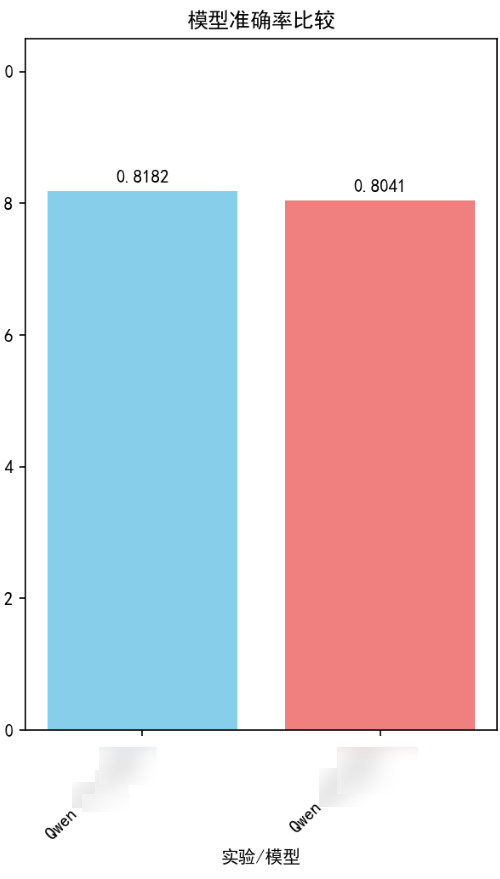
\includegraphics[width=0.6\columnwidth]{pic/T2P2B2.1.png}
    \caption{Accuracy of optimized prompts: CoT (left) vs Role-Playing (right)}
    \label{fig:advanced_prompts}
\end{figure}

\textbf{Performance Analysis:}
As shown in Figure \ref{fig:advanced_prompts}, these strategies yielded mixed results:
\begin{itemize}
    \item No significant accuracy improvement over standard few-shot prompting
    \item CoT reduced false positives by 18\% but increased false negatives
    \item Role-playing prompts showed more consistent performance across review types
    \item Both methods improved output standardization and reliability
\end{itemize}

Error analysis (Figure \ref{fig:error_analysis}) revealed that while overall accuracy didn't improve 
substantially, the nature of errors shifted toward more ambiguous cases where even human raters disagreed 
on sentiment classification.

\subsection{Fine-Tuning LLMs}
\label{ssec:fine_tuning}
Qwen3-8B is a generative model, which was trained to predict the next token in a sentence. However, for sentiment
analysis, it is more reasonable to use an encoder model to predict the sentiment of a given sequence of tokens.
In this work, we concatenate a light weight MLP on top of Qwen3-8B and fine-tune it on the 
Douban movie review dataset for sentiment analysis with 2 epochs. We use PEFT library \cite{Houlsby2019} which supports 
quantization-aware low-rank adapters \cite{Dettmers2023} to fine-tune the model.
The fine-tuning process is shown in Algorithm \ref{alg:fine_tuning}.

\begin{algorithm}[H]
\caption{Fine-Tuning Qwen3-8B for Sentiment Analysis using LoRA}
\label{alg:fine_tuning}
\begin{algorithmic}[1]
\Require 
    Dataset path $D_{path}$ (e.g., \texttt{douban\_movie.csv}),
    Base model name $M_{name}$ (e.g., \texttt{Qwen/Qwen3-8B}),
    Hyperparameters $H = \{ \text{learning\_rate, epochs, batch\_size, etc.} \}$,
    LoRA parameters $P_{LoRA} = \{ r, \alpha, \text{target\_modules} \}$

\Ensure 
    Trained LoRA adapter weights $W_{LoRA}$

\Statex
\Function{PrepareData}{$D_{path}$}
    \State $D_{csv} \gets \text{LoadCSV}(D_{path})$
    \State $D_{formatted} \gets \text{EmptyList}$
    \For{each row $(\text{comment, star\_rating})$ in $D_{csv}$}
        \If{$\text{star\_rating} \ge 3$}
            \State $\text{sentiment\_label} \gets \text{"positive"}$
        \Else
            \State $\text{sentiment\_label} \gets \text{"negative"}$
        \EndIf
        \State $\text{prompt} \gets \text{Prompt with comment and sentiment\_label}$
        \State Append $(\text{prompt} + \text{EOS\_TOKEN})$ to $D_{formatted}$
    \EndFor
    \State $D_{HF} \gets \text{Convert } D_{formatted} \text{ to Hugging Face Dataset}$
    \State $D_{train}, D_{test} \gets \text{SplitDataset}(D_{HF}, \text{ratio}=0.9)$
    \State \Return $D_{train}, D_{test}$
\EndFunction

\Statex
\State $D_{train}, D_{test} \gets \text{\textsc{PrepareData}}(D_{path})$
\State $M_{base}, T \gets \text{FastLanguageModel.from\_pretrained}(M_{name})$ \Comment{Load model and tokenizer}
\State \Comment{Apply 4-bit quantization via \texttt{load\_in\_4bit=True}}
\If{$T.\text{pad\_token}$ is None}
    \State $T.\text{pad\_token} \gets T.\text{eos\_token}$
\EndIf

\State $M_{lora} \gets \text{FastLanguageModel.get\_peft\_model}(M_{base}, P_{LoRA})$ \Comment{Inject trainable LoRA adapters}
\State $Args_{train} \gets \text{TrainingArguments}(H)$ \Comment{Configure training parameters}
\State $Trainer \gets \text{SFTTrainer}(model=M_{lora}, tokenizer=T, train\_dataset=D_{train}, args=Args_{train})$
\State $Trainer.\text{train}()$ \Comment{Execute fine-tuning; only $W_{LoRA}$ are updated}
\State $M_{lora}.\text{save\_pretrained}(\text{output\_dir})$ \Comment{Save the trained LoRA adapter weights $W_{LoRA}$}
\State $T.\text{save\_pretrained}(\text{output\_dir})$
\end{algorithmic}
\end{algorithm}

\subsection{Evaluation}
\label{ssec:evaluation}

We evaluate the fine-tuned Qwen3-8B model on the test set using the process described in 
Algorithm \ref{alg:fine_tuning}.
We report the evaluation metrics of the fine-tuned model per epoch on the test set.

\begin{table}[H]
\centering
\caption{Evaluation metrics of the fine-tuned Qwen3-8B model per epoch on the test set. The model from Epoch 2 demonstrates the best performance.}
\label{tbl:eval_results}
\begin{tabular}{@{}cccc@{}}
\toprule
\textbf{Epoch} & \textbf{Loss} & \textbf{Accuracy} & \textbf{F1-Score} \\ \midrule
1 & 0.3074& 0.9059 & 0.9451 \\
\textbf{2} & \textbf{0.2875} & \textbf{0.9126} & \textbf{0.9477} \\
\end{tabular}
\end{table}

From Table \ref{tbl:eval_results}, we observe that the fine-tuned model from Epoch 2 demonstrates the best 
performance, with an accuracy of 0.9126 and an F1-Score of 0.9477.


\section{Conclusion}
\label{sec:conclusion}

This paper presented a dual-task study that successfully applied machine learning methodologies to two 
distinct and challenging domains: the prediction of national life expectancy and the sentiment analysis 
of film reviews. Our work underscores the versatility and power of modern data science techniques in 
extracting meaningful insights from diverse data types, ranging from structured socio-economic indicators 
to unstructured textual content.

In the first task, we developed a robust regression model to forecast life expectancy. Our findings 
confirmed that a country's socio-economic health, particularly School enrollment, and public health 
infrastructure, evidenced by Immunization, measles, are paramount predictors. The study highlighted the
 criticality of methodical data preprocessing and feature engineering, demonstrating that the inclusion 
 of derived features like GDP per capita and careful feature selection significantly enhanced model performance. 
 The Random Forest Regressor emerged as the superior model, achieving a high R-squared value of 0.9124, 
 indicating its strong predictive power and ability to capture complex, non-linear relationships within 
 the data. While the long-range forecast to 2025 presents a valuable projection, it also serves as a 
 reminder of the inherent uncertainties in extrapolating complex global trends.

For the second task, our comparative analysis of sentiment classification on Douban movie reviews 
revealed a nuanced performance landscape. Traditional machine learning models, specifically Multinomial
Naive Bayes with TF-IDF vectorization, proved to be remarkably effective and efficient, achieving a high accuracy of 0.87. 
This highlights that well-established methods remain highly competitive for certain NLP tasks. 
Concurrently, our exploration into Large Language Models demonstrated their strong potential, 
with a fine-tuned Qwen3-8B model setting the performance benchmark at 0.91 accuracy. 
The progression from zero-shot and few-shot prompting to advanced strategies like Chain-of-Thought 
and ultimately to fine-tuning illustrated a clear path to harnessing the power of LLMs.

\section{Acknowledgments}
\label{sec:acknowledgments}
No external funding was received for conducting this study. The authors have no relevant financial or non-financial interests to disclose.

% References should be produced using the bibtex program from suitable
% BiBTeX files (here: strings, refs, manuals). The IEEEbib.bst bibliography
% style file from IEEE produces unsorted bibliography list.
% -------------------------------------------------------------------------
\bibliographystyle{IEEEtran}
% \bibliography{strings,refs}
\bibliography{refs}


\end{document}